\documentclass{article}
\usepackage{tikz}
\usetikzlibrary{positioning}

\begin{document}

\begin{figure}[h]
    \centering
    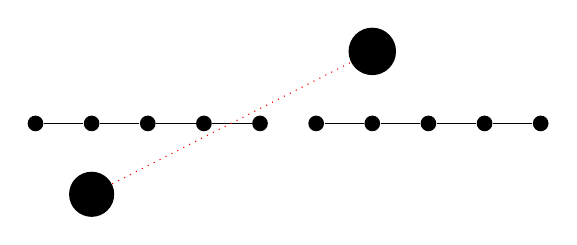
\begin{tikzpicture}[node distance=0.5cm]
        % Define nodes
        \node[circle,fill,inner sep=2pt] (u1) {};
        \node[circle,fill,inner sep=2pt,right=of u1] (u2) {};
        \node[circle,fill,inner sep=2pt,right=of u2] (u3) {};
        \node[circle,fill,inner sep=2pt,right=of u3] (u4) {};
        \node[circle,fill,inner sep=2pt,right=of u4] (u5) {};
        \node[circle,fill,inner sep=2pt,below=of u2] (ui) {$u_i$};
        
        \node[circle,fill,inner sep=2pt,right=of u5] (v1) {};
        \node[circle,fill,inner sep=2pt,right=of v1] (v2) {};
        \node[circle,fill,inner sep=2pt,right=of v2] (v3) {};
        \node[circle,fill,inner sep=2pt,right=of v3] (v4) {};
        \node[circle,fill,inner sep=2pt,right=of v4] (v5) {};
        \node[circle,fill,inner sep=2pt,above=of v2] (vj) {$v_j$};
        
        \draw (u1) -- (u2);
        \draw (u2) -- (u3);
        \draw (u3) -- (u4);
        \draw (u4) -- (u5);
        
        \draw (v1) -- (v2);
        \draw (v2) -- (v3);
        \draw (v3) -- (v4);
        \draw (v4) -- (v5);
        
        \draw[red,dotted] (ui) -- (vj);
    \end{tikzpicture}
    
    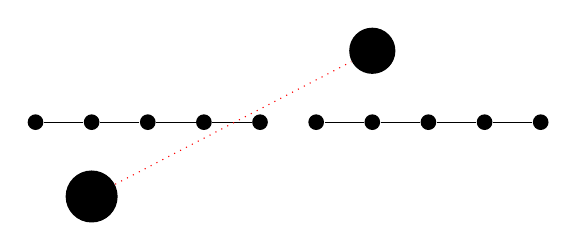
\begin{tikzpicture}[node distance=0.5cm]
        % Define nodes
        \node[circle,fill,inner sep=2pt] (w1) {};
        \node[circle,fill,inner sep=2pt,right=of w1] (w2) {};
        \node[circle,fill,inner sep=2pt,right=of w2] (w3) {};
        \node[circle,fill,inner sep=2pt,right=of w3] (w4) {};
        \node[circle,fill,inner sep=2pt,right=of w4] (w5) {};
        \node[circle,fill,inner sep=2pt,below=of w2] (wk) {$w_k$};
        
        \node[circle,fill,inner sep=2pt,right=of w5] (x1) {};
        \node[circle,fill,inner sep=2pt,right=of x1] (x2) {};
        \node[circle,fill,inner sep=2pt,right=of x2] (x3) {};
        \node[circle,fill,inner sep=2pt,right=of x3] (x4) {};
        \node[circle,fill,inner sep=2pt,right=of x4] (x5) {};
        \node[circle,fill,inner sep=2pt,above=of x2] (xl) {$x_\ell$};
        
        \draw (w1) -- (w2);
        \draw (w2) -- (w3);
        \draw (w3) -- (w4);
        \draw (w4) -- (w5);
        
        \draw (x1) -- (x2);
        \draw (x2) -- (x3);
        \draw (x3) -- (x4);
        \draw (x4) -- (x5);
        
        \draw[red,dotted] (wk) -- (xl);
    \end{tikzpicture}
    
    \caption{The subgraph in $G'_1$ formed by adding $(u_i,v_j)$ is isomorphic to the subgraph formed in $G'_2$ by adding $(w_k,x_\ell)$. Therefore, in the complements $G_1$ and $G_2$, removing those edges create isomorphic graphs.}
\end{figure}

\end{document}